\documentclass{beamer}
\usepackage{amsmath}
\usepackage{hyperref}
\usepackage{listings}
\usepackage{xcolor}
\hypersetup{colorlinks=true, citecolor=blue, filecolor=blue, linkcolor=blue, urlcolor=blue}
\definecolor{codegreen}{rgb}{0,0.6,0}
\definecolor{codegray}{rgb}{0.5,0.5,0.5}
\definecolor{codepurple}{rgb}{0.58,0,0.82}
\definecolor{backcolour}{rgb}{0.95,0.95,0.92}
 
\lstdefinestyle{mystyle}{
    backgroundcolor=\color{backcolour},   
    commentstyle=\color{codegreen},
    keywordstyle=\color{magenta},
    numberstyle=\tiny\color{codegray},
    stringstyle=\color{codepurple},
    basicstyle=\ttfamily\footnotesize,
    breakatwhitespace=false,         
    breaklines=true,                 
    captionpos=b,                    
    keepspaces=true,                 
    %numbers=left,                    
    numbersep=5pt,                  
    showspaces=false,                
    showstringspaces=false,
    showtabs=false,                  
    tabsize=2
}
 
\lstset{style=mystyle}

\mode<presentation> {

% The Beamer class comes with a number of default slide themes
% which change the colors and layouts of slides. Below this is a list
% of all the themes, uncomment each in turn to see what they look like.

%\usetheme{default}
\usetheme{AnnArbor}
%\usetheme{Antibes}
%\usetheme{Bergen}
%\usetheme{Berkeley}
%\usetheme{Berlin}
%\usetheme{Boadilla}
%\usetheme{CambridgeUS}
%\usetheme{Copenhagen}
%\usetheme{Darmstadt}
%\usetheme{Dresden}
%\usetheme{Frankfurt}
%\usetheme{Goettingen}
%\usetheme{Hannover}
%\usetheme{Ilmenau}
%\usetheme{JuanLesPins}
%\usetheme{Luebeck}
%\usetheme{Madrid}
%\usetheme{Malmoe}
%\usetheme{Marburg}
%\usetheme{Montpellier}
%\usetheme{PaloAlto}
%\usetheme{Pittsburgh}
%\usetheme{Rochester}
%\usetheme{Singapore}
%\usetheme{Szeged}
%\usetheme{Warsaw}

% As well as themes, the Beamer class has a number of color themes
% for any slide theme. Uncomment each of these in turn to see how it
% changes the colors of your current slide theme.

%\usecolortheme{albatross}
%\usecolortheme{beaver}
%\usecolortheme{beetle}
%\usecolortheme{crane}
%\usecolortheme{dolphin}
%\usecolortheme{dove}
%\usecolortheme{fly}
%\usecolortheme{lily}
%\usecolortheme{orchid}
%\usecolortheme{rose}
%\usecolortheme{seagull}
%\usecolortheme{seahorse}
%\usecolortheme{whale}
%\usecolortheme{wolverine}

%\setbeamertemplate{footline} % To remove the footer line in all slides uncomment this line
\setbeamertemplate{footline}[page number] % To replace the footer line in all slides with a simple slide count uncomment this line

\setbeamertemplate{navigation symbols}{} % To remove the navigation symbols from the bottom of all slides uncomment this line
}

\usepackage{graphicx} % Allows including images
\usepackage{booktabs} % Allows the use of \toprule, \midrule and \bottomrule in tables
%\usepackage {tikz}
\usepackage{tkz-graph}
\GraphInit[vstyle = Shade]
\tikzset{
  LabelStyle/.style = { rectangle, rounded corners, draw,
                        minimum width = 2em, fill = yellow!50,
                        text = red, font = \bfseries },
  VertexStyle/.append style = { inner sep=5pt,
                                font = \normalsize\bfseries},
  EdgeStyle/.append style = {->, bend left} }
\usetikzlibrary {positioning}
%\usepackage {xcolor}
\definecolor {processblue}{cmyk}{0.96,0,0,0}
%----------------------------------------------------------------------------------------
%	TITLE PAGE
%----------------------------------------------------------------------------------------

\title[Sampling Plans]{Numerical Optimization 13: Sampling Plans} %

\author{Qiang Zhu} % Your name
\institute[University of Nevada Las Vegas] % Your institution as it will appear on the bottom of every slide, may be shorthand to save space
{
University of Nevada Las Vegas\\ % Your institution for the title page
\medskip
}
\date{\today} % Date, can be changed to a custom date

\begin{document}

\begin{frame}
\titlepage % Print the title page as the first slide
\end{frame}

\begin{frame}
\frametitle{Overview} % Table of contents slide, comment this block out to remove it
\tableofcontents % Throughout your presentation, if you choose to use \section{} and \subsection{} commands, these will automatically be printed on this slide as an overview of your presentation
\end{frame}

%----------------------------------------------------------------------------------------
%	PRESENTATION SLIDES
%----------------------------------------------------------------------------------------

%------------------------------------------------

\section{Sampling}
\begin{frame}{Optimization with expensive function evaluations }
For many optimization problems, function evaluations can be quite expensive. 
\begin{itemize}
    \item an aircraft design may require a wind tunnel test
    \item deep learning hyperparameters may require a week of GPU training
    \item $\cdots$
\end{itemize} 
A common approach for optimizing in these contexts is to build a \textcolor{blue}{surrogate model},
Further evaluations of the true objective function can be used to improve the model. Fitting such models requires an initial set of points, ideally points that are space-filling; that is, points that cover the region as well as possible. 
\end{frame}

\section{Full Factorial}
\begin{frame}{Full Factorial}
The full factorial sampling plan places a grid of evenly spaced points over the search space.
\begin{itemize}
    \item a lower/upper-bound vector $a, b$ such that $a_i \leq x_i \leq b_i$
    \item $m_i$ samples in each $x_i$ separated by a distance $(b_i-a_i)/(m_i-1)$
\end{itemize} 
\begin{figure}
\centering
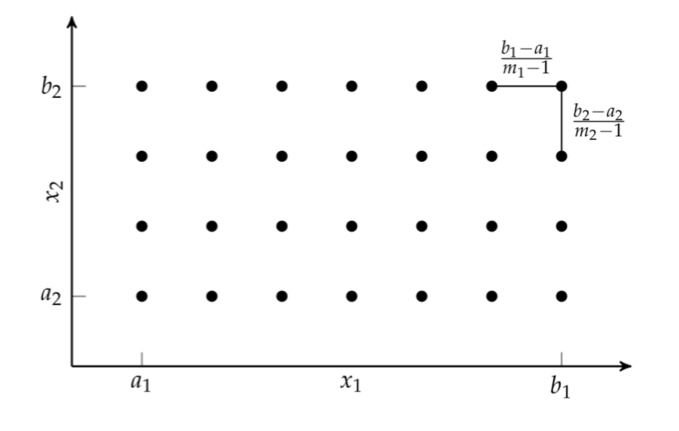
\includegraphics[width=80mm]{Figs/grid_search.jpeg}
\end{figure} 

\end{frame}

\section{Random Sampling}
\begin{frame}{Random Sampling}
In some cases, it may be possible to transform a problem so that constraints can be removed. For example, bound constraints a ≤ x ≤ b can be removed by passing x through a transform

\end{frame}


\section{Uniform Projection Plans}
\begin{frame}{Uniform Projection Plans}
A uniform projection plan with m samples on an $m \times m$ grid can be constructed using an $m$-element permutation. There are therefore $m!$ possible uniform projection plans.
\begin{figure}
\centering
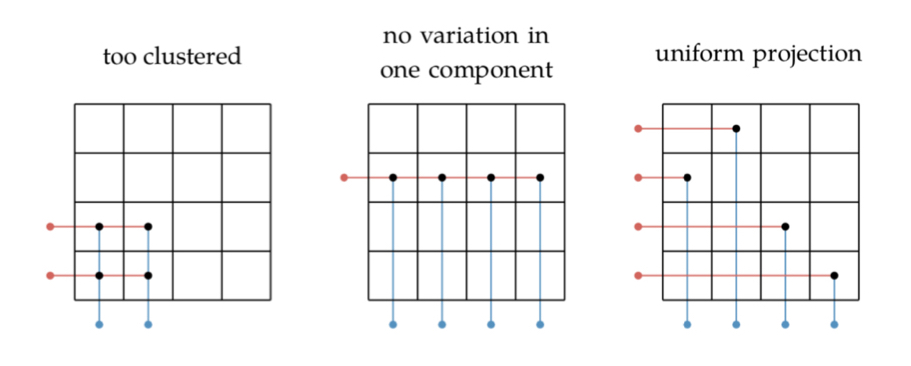
\includegraphics[width=120mm]{Figs/uni-proj.jpeg}
\end{figure} 
\end{frame}

\section{Stratified Sampling}
\begin{frame}{Uniform Projection Plans}
Stratified sampling modifies any grid-based sampling plan, including full factorial and uniform projection plans. Cells are sampled at a point chosen uniformly at random from within the cell rather than at the cell’s center。
\begin{figure}
\centering
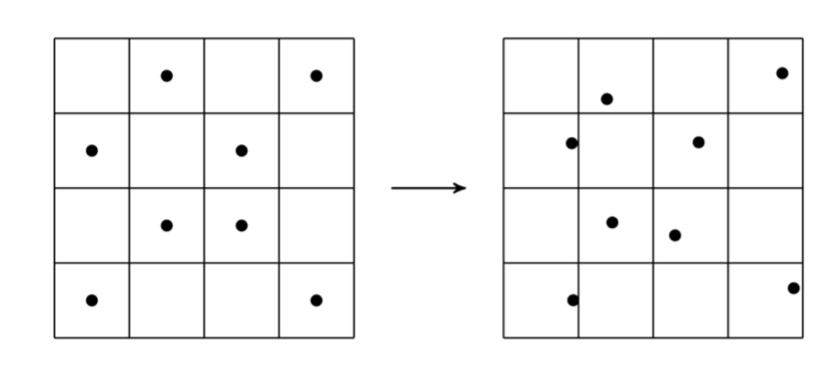
\includegraphics[width=120mm]{Figs/strafied.jpeg}
\end{figure} 
\end{frame}


\section{Space-Filling Metrics}
\begin{frame}{Space-Filling Metrics}
A good sampling plan fills the design space since the ability for a surrogate model to generalize from samples decays with the distance from those samples. Not all plans, even uniform projection plans, are equally good at covering the search space. 
\begin{itemize}
    \item Discrepancy, the maximum difference between the fraction of samples in a hyper-rectangular subset H and that subset’s volume:
    \begin{equation*}
        d(X) = \underset{H}{\sup} |\frac{\#X\cap H}{\#X} - \lambda(H)|
    \end{equation*}
    where $\#X$ and $\#X \cap H$ are the numbers of $X$ points and $X$ in $H$. 
    \item Pairwise Distances between all points within each sampling plan
    
\end{itemize}


\end{frame}

\section{Quasi-Random Sequences}
\begin{frame}{Quasi-Random Sequences}
Quasi-random sequences are often used in the context of trying to approximate an integral over a multidimensional space:
\begin{equation*}
    \int_\chi f(\boldsymbol{x})d\boldsymbol{x} \approx \frac{v}{m}\sum_{i=1}^m f(\boldsymbol{x}^i)
\end{equation*}
where each $\boldsymbol{x}^i$ is sampled uniformly at random over the domain $X$ and $v$ is the volume of $\boldsymbol{\chi}$ .

Quasi-random sequences are deterministic sequences that fill the space in a systematic manner so that the integral converges as fast as possible in the number of points $m$. They are typically constructed for the unit n-dimensional hypercube with the following methods.
\begin{itemize}
    \item Additive Recurrence
    \item Halton Sequence
    \item Sobol Sequence
\end{itemize}
\end{frame}

\begin{frame}{Additive Recurrence}
Quasi-random sequences are often used in the context of trying to approximate an integral over a multidimensional space:
\begin{equation*}
    x^{k+1} = x^k + c ~~~(\mod 1)
\end{equation*}
produce space-filling sets provided that $c$ is irrational. The value of $c$ leading to
\begin{equation*}
    c = 1 - \Phi = \frac{\sqrt{5}-1}{2} = 0.618
\end{equation*}
where $\Phi$ is the golden ratio.
We can construct a space-filling set over $n$ dimensions using an additive recurrence sequence for each coordinate, each with its own value of $c$. The square roots of the primes are known to be irrational, and can thus be used to obtain different sequences for each coordinate:
\begin{equation*}
    c_1 =\sqrt{2}, ~c_2 =\sqrt{3}, ~c_3 =\sqrt{5}, c_4 =\sqrt{7}, c_5 =\sqrt{11},
\end{equation*}
\end{frame}

\begin{frame}{Halton Sequence}
\textcolor{blue}{Radical Inversion}
\begin{equation*}
\begin{split}
    i & = \sum_{k=0}^{M-1} a_k(i)b^k \\
\Psi_{b, C} &= (b^{-1}, \cdots, b^{-M}) [C (a_0(i), \cdots, a_M(i) )^T]   
\end{split}
\end{equation*}
where $b$ is the \textcolor{blue}{base number}, and $C$ is the \textcolor{blue}{generator matrix}. When $C$ is the identity matrix, it is called \textcolor{blue}{van der Corput sequences},
\begin{itemize}
    \item $b$ = 2 
    \begin{equation*}
        X = \bigg\{ \frac{1}{2}, \frac{1}{4}, \frac{3}{4}, \frac{1}{8}, \frac{5}{8}, \frac{3}{8}, \frac{7}{8}, \frac{1}{16}, \cdots \bigg\}
    \end{equation*}
    \item $b$ = 5 
    \begin{equation*}
        X = \bigg\{ \frac{1}{5}, \frac{2}{5}, \frac{3}{5}, \frac{4}{5}, \frac{1}{25}, \frac{6}{25}, \frac{11}{25}, \cdots \bigg\}
    \end{equation*}
\end{itemize}

Halton Sequence uses coprime numbers in order to be uncorrelated. 

\end{frame}

\begin{frame}{Sobol Sequence}
In the Sobol sequence, each dimension uses the base 2 with different $C$.
\begin{figure}
\centering
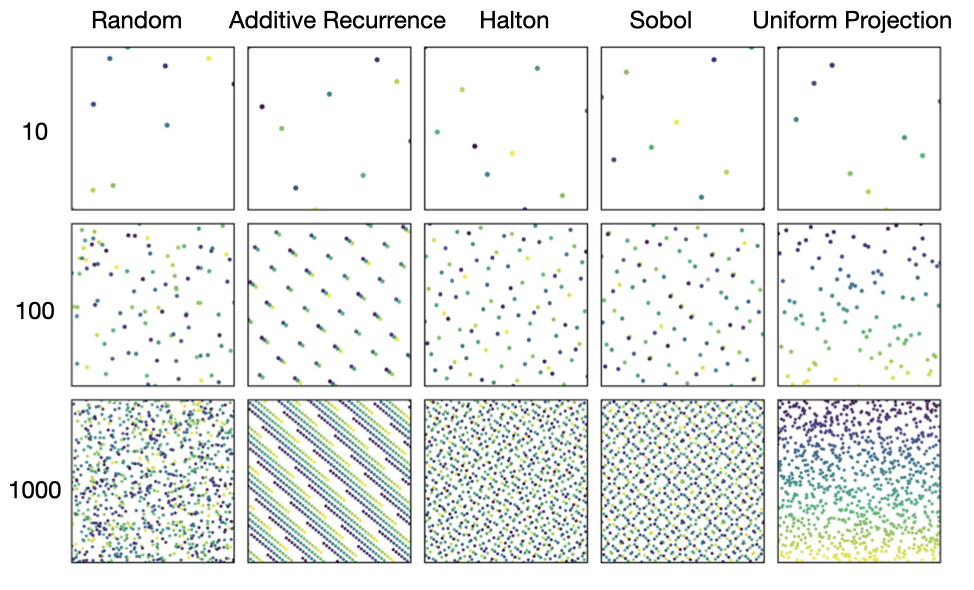
\includegraphics[width=120mm]{Figs/sample_all.jpeg}
\end{figure} 



\end{frame}


\section{Summary}
\begin{frame}{Summary}
    \begin{itemize}
        \item Sampling plans are used to cover search spaces with a limited number of points.
        \item Full factorial sampling, which involves sampling at the vertices of a uniformly discretized grid, requires a number of points exponential in the number of dimensions.
        \item Uniform projection plans,which project uniformly over each dimension,can be efficiently generated and can be optimized to be space filling.
        \item Quasi-random sequences are deterministic procedures by which space-filling sampling plans can be generated.
    \end{itemize}
    
\end{frame}
\end{document}

